%%%%%%%%%%%%%%%%%%%%%%%%%%%%%%%%%%%%%%%%%
% Wenneker Article
% LaTeX Template
% Version 2.0 (28/2/17)
%
% This template was downloaded from:
% http://www.LaTeXTemplates.com
%
% Authors:
% Vel (vel@LaTeXTemplates.com)
% Frits Wenneker
%
% License:
% CC BY-NC-SA 3.0 (http://creativecommons.org/licenses/by-nc-sa/3.0/)
%
%%%%%%%%%%%%%%%%%%%%%%%%%%%%%%%%%%%%%%%%%

%----------------------------------------------------------------------------------------
%	PACKAGES AND OTHER DOCUMENT CONFIGURATIONS
%----------------------------------------------------------------------------------------

\documentclass[10pt, a4paper, twocolumn]{article} % 10pt font size (11 and 12 also possible), A4 paper (letterpaper for US letter) and two column layout (remove for one column)



%%%%%%%%%%%%%%%%%%%%%%%%%%%%%%%%%%%%%%%%%
% Wenneker Article
% Structure Specification File
% Version 1.0 (28/2/17)
%
% This file originates from:
% http://www.LaTeXTemplates.com
%
% Authors:
% Frits Wenneker
% Vel (vel@LaTeXTemplates.com)
%
% License:
% CC BY-NC-SA 3.0 (http://creativecommons.org/licenses/by-nc-sa/3.0/)
%
%%%%%%%%%%%%%%%%%%%%%%%%%%%%%%%%%%%%%%%%%

%----------------------------------------------------------------------------------------
%	PACKAGES AND OTHER DOCUMENT CONFIGURATIONS
%----------------------------------------------------------------------------------------

\usepackage{hyperref}

\hypersetup{
    colorlinks=true,
    linkcolor=blue,
    filecolor=magenta,      
    urlcolor=cyan,
    pdftitle={Overleaf Example},
    pdfpagemode=FullScreen,
    }
    
\urlstyle{same}

\usepackage[english]{babel} % English language hyphenation

\usepackage{microtype} % Better typography

\usepackage{amsmath,amsfonts,amsthm} % Math packages for equations

\usepackage[svgnames]{xcolor} % Enabling colors by their 'svgnames'

\usepackage[hang, small, labelfont=bf, up, textfont=it]{caption} % Custom captions under/above tables and figures

\usepackage{booktabs} % Horizontal rules in tables

\usepackage{lastpage} % Used to determine the number of pages in the document (for "Page X of Total")

\usepackage{graphicx} % Required for adding images

\usepackage{enumitem} % Required for customising lists

\setlist{noitemsep} % Remove spacing between bullet/numbered list elements

\usepackage{sectsty} % Enables custom section titles
\allsectionsfont{\usefont{OT1}{phv}{b}{n}} % Change the font of all section commands (Helvetica)

%----------------------------------------------------------------------------------------
%	MARGINS AND SPACING
%----------------------------------------------------------------------------------------

\usepackage{geometry} % Required for adjusting page dimensions

\geometry{
	top=1cm, % Top margin
	bottom=1.5cm, % Bottom margin
	left=2cm, % Left margin
	right=2cm, % Right margin
	includehead, % Include space for a header
	includefoot, % Include space for a footer
	%showframe, % Uncomment to show how the type block is set on the page
}

\setlength{\columnsep}{7mm} % Column separation width

%----------------------------------------------------------------------------------------
%	FONTS
%----------------------------------------------------------------------------------------

\usepackage[T1]{fontenc} % Output font encoding for international characters
\usepackage[utf8]{inputenc} % Required for inputting international characters

\usepackage{XCharter} % Use the XCharter font

%----------------------------------------------------------------------------------------
%	HEADERS AND FOOTERS
%----------------------------------------------------------------------------------------

\usepackage{fancyhdr} % Needed to define custom headers/footers
\pagestyle{fancy} % Enables the custom headers/footers

\renewcommand{\headrulewidth}{0.0pt} % No header rule
\renewcommand{\footrulewidth}{0.4pt} % Thin footer rule

\renewcommand{\sectionmark}[1]{\markboth{#1}{}} % Removes the section number from the header when \leftmark is used

%\nouppercase\leftmark % Add this to one of the lines below if you want a section title in the header/footer

% Headers
\lhead{} % Left header
\chead{\textit{\thetitle}} % Center header - currently printing the article title
\rhead{} % Right header

% Footers
\lfoot{} % Left footer
\cfoot{} % Center footer
\rfoot{\footnotesize Page \thepage\ of \pageref{LastPage}} % Right footer, "Page 1 of 2"

\fancypagestyle{firstpage}{ % Page style for the first page with the title
	\fancyhf{}
	\renewcommand{\footrulewidth}{0pt} % Suppress footer rule
}

%----------------------------------------------------------------------------------------
%	TITLE SECTION
%----------------------------------------------------------------------------------------

\newcommand{\authorstyle}[1]{{\large\usefont{OT1}{phv}{b}{n}\color{DarkRed}#1}} % Authors style (Helvetica)

\newcommand{\institution}[1]{{\footnotesize\usefont{OT1}{phv}{m}{sl}\color{Black}#1}} % Institutions style (Helvetica)

\usepackage{titling} % Allows custom title configuration

\newcommand{\HorRule}{\color{DarkGoldenrod}\rule{\linewidth}{1pt}} % Defines the gold horizontal rule around the title

\pretitle{
	\vspace{-30pt} % Move the entire title section up
	\HorRule\vspace{10pt} % Horizontal rule before the title
	\fontsize{32}{36}\usefont{OT1}{phv}{b}{n}\selectfont % Helvetica
	\color{DarkRed} % Text colour for the title and author(s)
}

\posttitle{\par\vskip 15pt} % Whitespace under the title

\preauthor{} % Anything that will appear before \author is printed

\postauthor{ % Anything that will appear after \author is printed
	\vspace{10pt} % Space before the rule
	\par\HorRule % Horizontal rule after the title
	\vspace{20pt} % Space after the title section
}

%----------------------------------------------------------------------------------------
%	ABSTRACT
%----------------------------------------------------------------------------------------

\usepackage{lettrine} % Package to accentuate the first letter of the text (lettrine)
\usepackage{fix-cm}	% Fixes the height of the lettrine

\newcommand{\initial}[1]{ % Defines the command and style for the lettrine
	\lettrine[lines=3,findent=4pt,nindent=0pt]{% Lettrine takes up 3 lines, the text to the right of it is indented 4pt and further indenting of lines 2+ is stopped
		\color{DarkGoldenrod}% Lettrine colour
		{#1}% The letter
	}{}%
}

\usepackage{xstring} % Required for string manipulation

\newcommand{\lettrineabstract}[1]{
	\StrLeft{#1}{1}[\firstletter] % Capture the first letter of the abstract for the lettrine
	\initial{\firstletter}\textbf{\StrGobbleLeft{#1}{1}} % Print the abstract with the first letter as a lettrine and the rest in bold
}

%----------------------------------------------------------------------------------------
%	BIBLIOGRAPHY
%----------------------------------------------------------------------------------------

\usepackage[backend=bibtex,style=authoryear,natbib=true]{biblatex} % Use the bibtex backend with the authoryear citation style (which resembles APA)

\addbibresource{example.bib} % The filename of the bibliography

\usepackage[autostyle=true]{csquotes} % Required to generate language-dependent quotes in the bibliography
 % Specifies the document structure and loads requires packages

%----------------------------------------------------------------------------------------
%	ARTICLE INFORMATION
%----------------------------------------------------------------------------------------

\title{REU in Data Science: Creating and Maintaining Expectations at HBCU University} % The article title

\author{
	\authorstyle{Yohn Jairo Parra Bautista, PhD\textsuperscript{1} and Carlos Theran\textsuperscript{1} and Richard Alo, PhD\textsuperscript{1}} % Authors
	\newline\newline % Space before institutions
	\textsuperscript{1}\institution{Florida A\&M University, Tallahassee, United States of America}\\ % Institution 1
}

% Example of a one line author/institution relationship
%\author{\newauthor{John Marston} \newinstitution{Universidad Nacional Autónoma de México, Mexico City, Mexico}}

\date{\today} % Add a date here if you would like one to appear underneath the title block, use \today for the current date, leave empty for no date

%----------------------------------------------------------------------------------------

\begin{document}

\maketitle % Print the title

\thispagestyle{firstpage} % Apply the page style for the first page (no headers and footers)

%----------------------------------------------------------------------------------------
%	ABSTRACT
%----------------------------------------------------------------------------------------

% \lettrineabstract{Research Experience for Undergraduates (REU) at HBCU University brings challenges while lift up expectations in participants. The approach model is located in the hearth of algorithms, datasets and computer power. Florida A\&M University start first time an REU program in Data Science with the intention to advocated and mentor minority population in the era of Machine Learning and AI.}

\lettrineabstract{Research Experience for Undergraduates (REU) at HBCU University brings challenges while lifting up expectations in participants. The approaching model is located in the heart of hands-on application on algorithms, datasets, and computer power. Florida A\&M University starts an REU program in Data Science intending to advocate and mentor minority populations in the era of Machine Learning and AI. This experience involves an interdisciplinary group of undergraduate students from different majors such as; Computer Science and Information Technology,  Biology Pre-Medicine, Mathematics, Software Engineer, Pharmacy, Biology Pre-Dental, Computer Engineering, Computer Science, Biology, Mathematical Sciences. At the end of the program, the students could integrate AI, machine learning, and deep learning techniques to provide real solutions to their research projects in their area. For example, Time Series Analysis of Blockchain-Based Cryptocurrency, Analyzing the Advantages and Disadvantages of Artificial Intelligence for Breast Cancer Detection in Women, Analysis of Autism in three different cities using AI, among others projects, which were leverage into students' GitHub Repositories. The students who participated in the REU indicated that this was very important and useful for their careers.  They reported significant enhancement of essential cognitive and personal skills, among the enumerable learned skills, can be mention python programming, skit-learn packets to build machine learning models, the use of Git & Github as version control system collaborating work.} 

%----------------------------------------------------------------------------------------
%	ARTICLE CONTENTS
%----------------------------------------------------------------------------------------

\section{What is an REU Data Science Research Group? }

REU in Data Science is an experience which faculty, speakers and undergraduate students enjoy an environment designed to learn by doing.  \citep{Reference1}. Most universities and colleges offer their science majors the opportunity to gain some sort of research experience\citep{Reference1,Reference2}. However, Data Science offers a hands on approach to any student that wants to experiment with data, algorithms and programming. Over a one-year project period, Florida A\&M University start a computational data science program that offers courses like python, R and machine learning across campus.  The Data science REU students have diverse backgrounds and experiences and major in different fields. Gender population in Figure \ref{gender}. Major distribution vs GPA in Figure \ref{major}.

We advertised our REU Data Science Site program via a variety of channels including email distributions to targeted institutions, a variety of list serves, and personal contacts. In the first recent month 2021 program, we received 30 applications from across the alliance in Florida, among which 23 were complete with all required documents, including the application form, purpose statement, resume, unofficial transcript, and two letters of references. Based on a comprehensive rubric, the 23 applicants were selected to participate in our Summer 2021 program.

\begin{figure}
	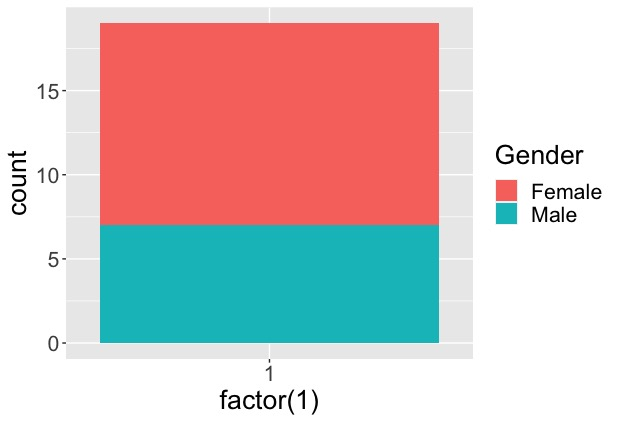
\includegraphics[width=\linewidth]{gender.jpeg} % Figure image
	\caption{REU Gender Distribution} % Figure caption
	\label{gender} % Label for referencing with \ref{bear}
\end{figure}

\begin{figure}
	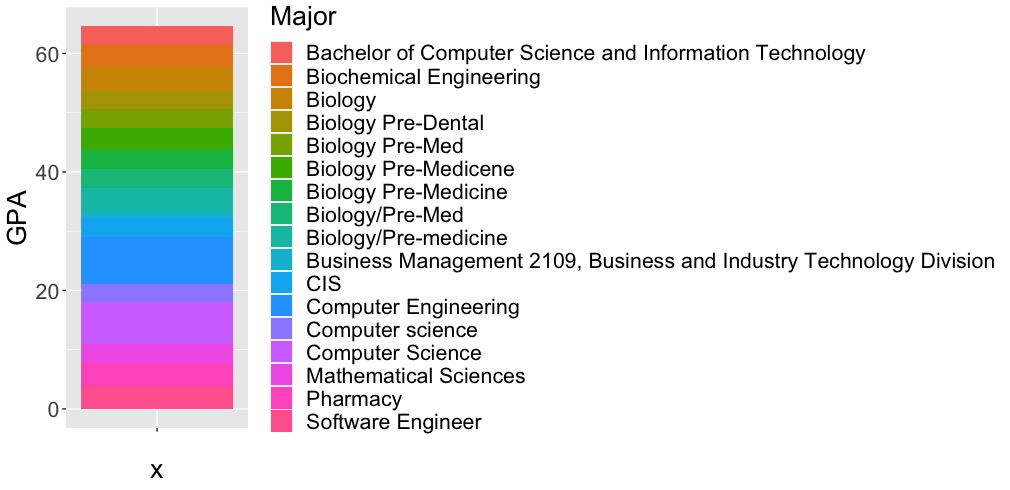
\includegraphics[width=\linewidth]{major1.jpeg} % Figure image
	\caption{REU Major Distribution vs GPA} % Figure caption
	\label{major} % Label for referencing with \ref{bear}
\end{figure}

We have the first REU in Data Science at Florida A\&M University, which excels the expectations of students and audience. The modality of learning is project based with the student centric approach. We delivered recorded lectures, speakers from Microsoft, Indiana University and engaging activities to boost students curiosity. Students share their curiosity through the ability to find their own societal problems that required responsible AI and ML. Public datasets was showing to the students but that do not stop the desire to collect their own data. REU Data Science students participate in a mix of activities particularly designed to improve their curiosity with an inductive research (i.e., find patterns in data to target hypothesis questions). We have a teamwork and communication skills through the benefits of new technology. Table I shows the overall schedule of the 8-week summer activities of the REU Site program, which are described in the following subsection.

\begin{table}
	\caption{Overall Schedule of REU Data Science 8-week summer activities}
	\centering
	\begin{tabular}{llr}
		\toprule
		\multicolumn{2}{c}{Activities} \\
		\cmidrule(r){1-2}
		Month Number & 1 & 2  \\
		\midrule
		Orientation & X &  \\
		Speakers & X &  \\
		Focus Group & X & X \\
		Project details & X & X \\
		Weekly Data Science Tips & X & X \\
		Final Presentation &  & X \\
		\bottomrule
	\end{tabular}
\end{table}
%------------------------------------------------

\subsection{REU Data Science Research Group Components}

We conducted an orientation to introduce the REU data science program activities and all faculty, staff, and graduate students involved.
Particularly, we conveyed what the REU data science was designed to students who were expected to accomplish a project by the end of the 8-week program.

Table 2 summarizes the Data Science Research Group Components(DSRG's) and the benefits of incorporating those components from industry, faculty mentor and students perspectives.


Speakers: We have a total of 6 speakers during the first month, which contextualized with industry the topics we taught. speakers from Microsoft emphasized the importance to find local problems with local data. We as a data scientists we assume the need of data that is not available for us. However, data have to come with a real world problem. Some examples of courses should be taught in academia are:

\begin{itemize}
	\item Data Prep 
	\item Cloud Computing 
	\item Python and R for Data Science
\end{itemize}


\section{REU students' Projects}

REU Data Science Research Projects: We have each student providing a research topic and data based on their majors. Each REU student is mentored by a faculty mentor and a graduate student. Some interesting projects are:


\subsection{Time Series Analysis of Blockchain-Based Cryptocurrency Price Changes}
This project applies neural networks and Artificial Intelligence (AI) to historical records of high-risk cryptocurrency coins to train a prediction model that guesses their price.  


\begin{description}
	\item[First] Project: Time Series Analysis of Blockchain-Based Cryptocurrency Price Changes, Jacques Fleischer
	\item[Second] Project: Breast Cancer and Genetics, Kehinde Ezekiel
	\item[Third] Project: AI in Orthodontics, Whitney McNair
	\item[Fourth] Project: Object Recognition, David Umanzor
	\item[Five] Project: Cyber Attacks Detection Using AI Algorithms, Victor Adankai
	\item[Six]  Project: Handwriting Recognition Using AI, Mikahla Reeves
	\item[Seventh] Project: Increasing Cervical Cancer Risk Analysis, Theresa Jeanbaptiste
	\item[Eight] Project: Aquatic Animals Classification Using AI, Timia Williams
	\item[Ninth] Project: Detecting Multiple Sclerosis Symptoms using AI, Raeven Hatcher
	\item[Tenth] Project: Analysing Hashimoto disease causes using AI, Sheimy Paz
	\item[Eleventh] Project: Analysis of Covid-19 Vaccination Rates in Different Races, Ololade Latinwo
	\item[Twelve] Project: AI and Dentronics, Jamyla Young
	\item[Thirteen] Project: Analyzing the Advantages and Disadvantages of Artificial Intelligence for Breast Cancer 
	\item[Last] Project: Analysis of Autism in three different cities using AI, Myra Saunders
\end{description}

\begin{table}
\centering
\caption{Data Science Research Group Components}
\begin{tabular}{|c|c|} \hline
Data Science Research Group Components&Traditional Hierarchical Research Models\\ \hline
Collaboration between students, mentors and industry & Collaboration is often between students and mentors\\ \hline
Different backgrounds is encouraged regardless the programming skills & \\ \hline
 &  \\ \hline
\hline\end{tabular}
\end{table}

%------------------------------------------------




\section{REU Data Science Research Group as a Transformative Experience}


Research projects are the key component of our first REU in data science. We provide REU students a fair research experience, we have designed the research projects that students can select their data and problem with common intellectual focus on self-motivation in Data Science education. Transformative experience in Data Science explains weaknesses in many digital transformation strategy efforts and how data can address the problem a certain level. Students report their weaknesses with a tutorial they explain in class and share with peers. 



%----------------------------------------------------------------------------------------
%	BIBLIOGRAPHY
%----------------------------------------------------------------------------------------

\printbibliography[title={Bibliography}] % Print the bibliography, section title in curly brackets

%----------------------------------------------------------------------------------------

\end{document}
